\documentclass[11pt,letterpaper]{article}
\usepackage[top=1in,bottom=1in,left=1in,right=1in]{geometry}
\pagestyle{empty}
\usepackage{graphicx}
\usepackage{amsmath}

\usepackage[dvipsnames]{xcolor}
%\newcommand{\sol}[1]{{\color{NavyBlue} #1}}
\newcommand{\sol}[1]{{\color{White} #1}} % uncomment to hide solutions


\begin{document}
\setlength{\parindent}{0cm}
\setlength{\parskip}{11pt}
Exam \#2: Dynamics, momentum, and energy

Name: \hfill /30\\

\hrulefill\\
1. A child rides a sled down a hill and onto level ground at the bottom of the hill, eventually coming
to a stop when she bumps into a tree. Sketch the kinetic energy, gravitational potential energy, and thermal energy of the system as functions of the child's position. Include the child and the ground in the system, and assume that the coefficient of friction between the sled and the snow is constant. [6 pts]

%\sol{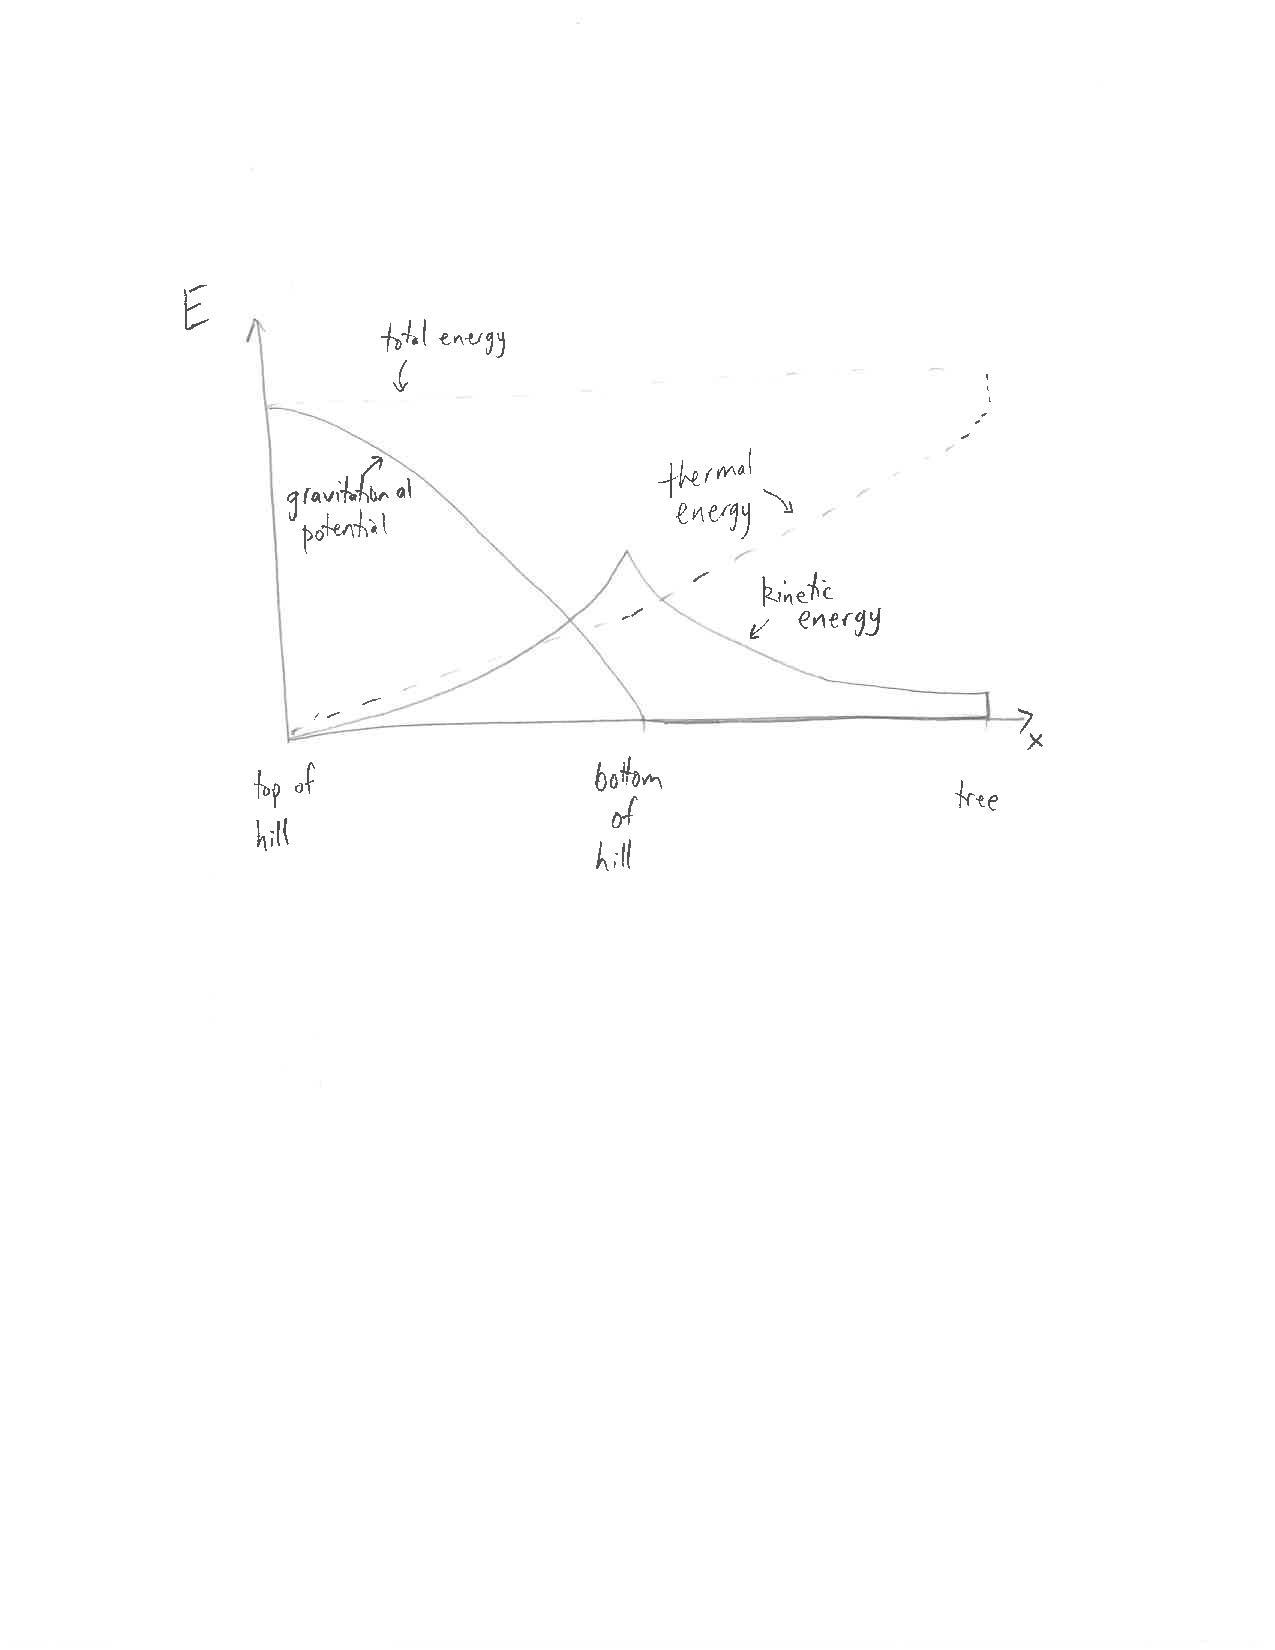
\includegraphics[trim={2cm 10cm 2cm 3cm}, clip, width=\textwidth]{./exam2_1_sol.pdf}}



\clearpage
2. A man claims that he can safely hold on to a 10.0~kg child in a head-on collision with a relative speed of 50~m/s (close to 200~km/h or 120~mph). Assume that the collision takes 0.1~s. Find the magnitude of the average force that would be needed to hold onto the child. Is it possible for a person to apply that sort of force (justify your answer)? [6 pts]

\sol{This is an impulse-momentum problem.
$$\vec{J} = \Delta \vec{p}$$
Since it is a one-dimensional problem, we can drop the vectors, but keep in mind that the sign of the velocity (and momentum) still matters. Let's assume that the car is traveling in the positive direction.
$$J = mv_f - mv_i$$
Assuming that the man is able to hold onto the child, the final velocity is $v_f=0$, which means that the impulse is
$$J = -mv_i = -500\mbox{ N}\cdot\mbox{s}$$
Impulse is defined as
$$J=F_{avg}\Delta t,$$
and therefore
$$F_{avg}=\frac{J}{\Delta t} \rightarrow \boxed{F_{avg} = -5000\mbox{ N}}$$
The negative sign indicates that the force is pointing in the negative x-direction.

For comparison, a 100~kg person has a weight (gravitational force) of just under 1000~N. The average force necessary to hold onto the child is five times this value, and the maximum force will be even larger. This is not feasible.

} 






\clearpage
3. A railroad car of mass $2.00\times 10^4$~kg moving at 3.00~m/s collides and couples with two coupled railroad cars, each of the same mass as the single car and moving in the same direction at 1.20~m/s. 

(a) What is the speed of three coupled cars after the collision? [3 pts]

\sol{Using conservation of momentum and denoting the cars masses as $m$ and $2m$:
$$P_i = P_f$$
$$mv_1 + 2mv_2 = 3mv_f$$
$$v_1+2v_2 = 3v_f \rightarrow v_f = \frac{1}{3}(v_1+2v_2)$$
$$\boxed{v_f = 1.80 \mbox{ m/s}}$$ 
}

\vspace{2cm}
(b) How much thermal energy was generated during the collision? [3 pts]

\sol{Using conservation of energy,
$$\Delta E = \Delta K + \Delta E_{th} = 0$$
$$\Delta E_{th} = -\Delta K$$
$$\Delta E_{th} = K_i - K_f = \frac{1}{2}mv_1^2 + \frac{1}{2}(2m)v_2^2 - \frac{1}{2}(3m)v_f^2$$
$$\boxed{\Delta E_{th} = 21600\mbox{ J}}$$
This is about 18\% of the kinetic energy prior to the collision.

}




\clearpage
4. Two objects of masses $m_1=0.5$~kg and $m_2=1.0$~kg are placed on a horizontal frictionless surface. A spring with spring constant $k=300$~N/m placed between them and compressed by 0.1~m. The spring is not attached to either mass. The masses are released and shoot outward, as shown in the diagram below. Ignore the mass of the spring. Determine $\vec{v}_1$ and $\vec{v}_2$. [6 pts]

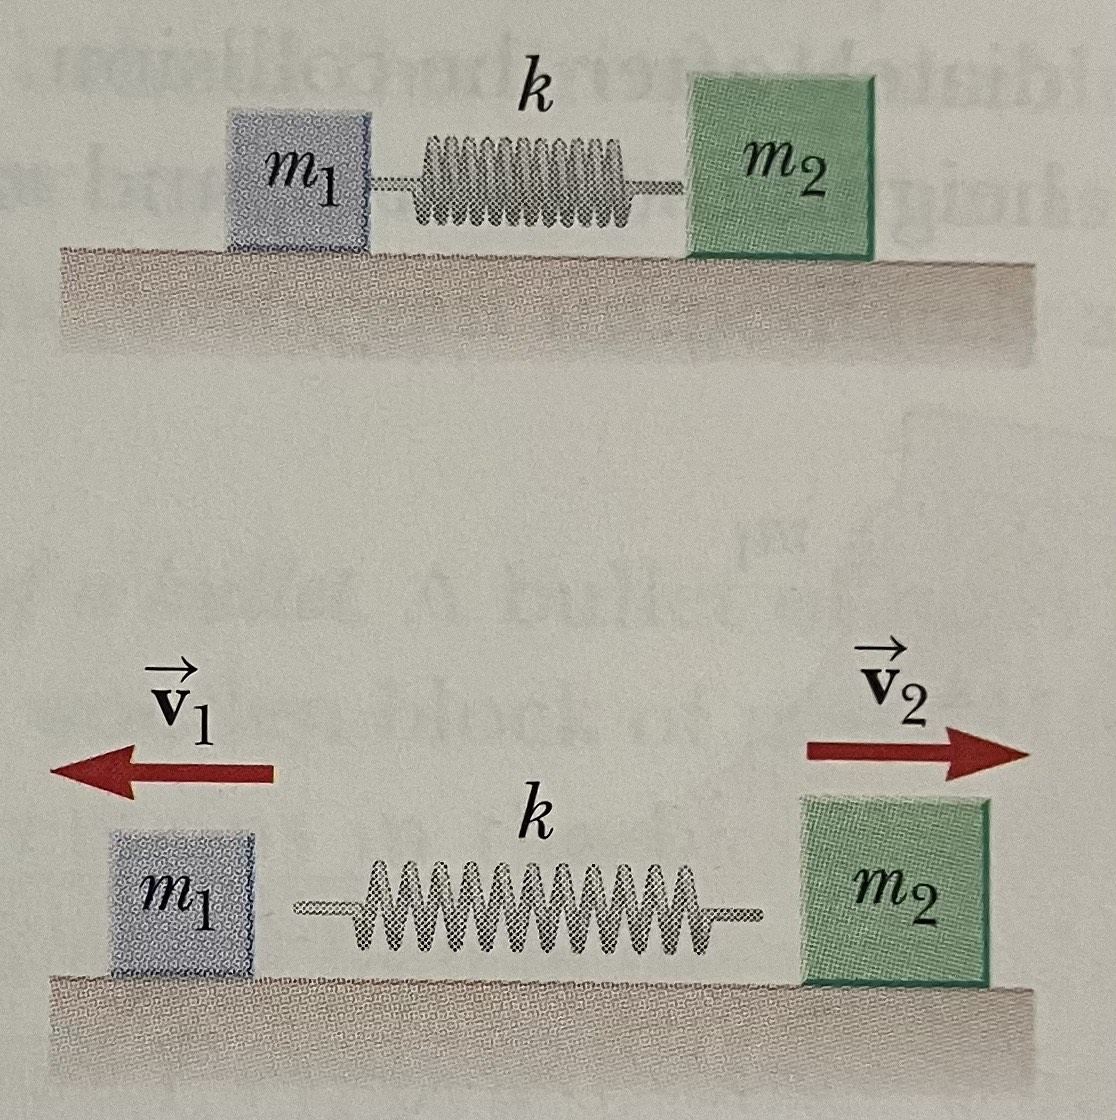
\includegraphics[width=8cm]{./exam2_4.jpg}

\sol{This problem requires conservation of momentum and conservation of energy. 

Using conservation of momentum, we can write
$$P_i = P_f$$
$$0 = -m_1v_1 + m_2v_2 \Rightarrow v_1 = \frac{m_2}{m_1}v_2$$
where I am treating $v_1$ as a positive number and including a negative sign to indicate the direction. It is clear that $\vec{v}_1$ and $\vec{v}_2$ must point in opposite directions if momentum will be conserved.

Using conservation of energy, we can write
$$\Delta E = 0 = \Delta K + \Delta U_s$$
$$0 = K_f-K_i + U_{s,f}-U_{s,i} = K_f - U_{s,i}$$
$$0 = \frac{1}{2}m_1v_1^2 + \frac{1}{2}m_2v_2^2 - \frac{1}{2}kx_i^2$$ 
Multiplying both sides by 2 and substituting in the expression for $v_1$ from above,
$$0 = \frac{m_2^2}{m_1}v_2^2+m_2v_2^2 - kx_i^2 = m_2v_2^2\left(1+\frac{m_2}{m_1}\right) - kx_i^2$$
$$ v_2 = x_i\sqrt{k\left(\frac{m_1}{m_2(m_1+m_2)}\right)} \rightarrow \boxed{\vec{v}_2=1.0\mbox{ m/s}}$$
Plugging back into the result for $v_1$,
$$\boxed{\vec{v}_1=-2.0\mbox{ m/s}}$$

}

\clearpage
5. Two objects, with masses $m_1$ and $m_2$ , are supported by narrow posts as shown in the figure below. Calculate the normal forces acting on each of the posts. Ignore the width of the posts, and therefore assume that the normal forces are acting on the outside edges of the posts. [6 pts]

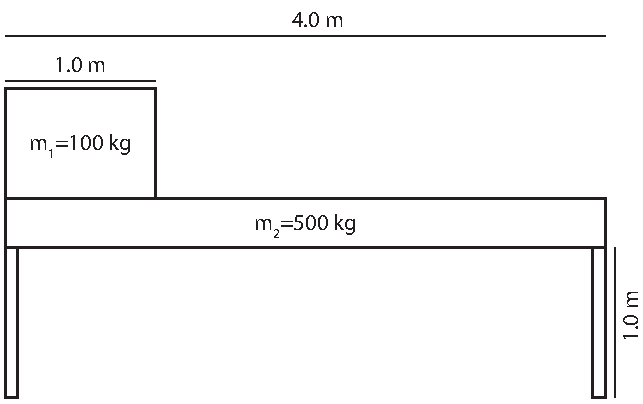
\includegraphics[width=8cm]{./exam2_5.pdf}

\sol{Let $L=4.0$~m. Summing the torques around the left edge,
$$\sum \tau = N_2L - m_2g\frac{L}{2} - m_1g\frac{L}{8} = 0$$
$$N_2 = \frac{1}{2}m_2g+\frac{1}{8}m_1g = \boxed{N_2 = 2575\mbox{ N}}$$

Now summing the torques around the right edge,
$$\sum \tau = -N_1L + m_2g\frac{L}{2} + m_1g\frac{7L}{8} = 0$$
$$N_1 = \frac{1}{2}m_2g + \frac{7}{8}m_1g = \boxed{N_1 = 3311 \mbox{ N}}$$

You could have also combined one of these with a force balance equation,
$$\sum F_y = N_1+N_2-m_1g-m_2g = 0,$$
and arrived at the same answers.

}





\end{document}


